\documentclass{article}
\usepackage[ngerman]{babel}
\usepackage{graphicx}
\usepackage{subcaption}
\usepackage{acro}
\usepackage{pdfpages}
\usepackage{doi}

\usepackage[backend=biber,style=numeric,doi=true,url=true]{biblatex}
\addbibresource{literatur.bib}


\title{Echtzeitfähige Deep-Learning-basierte Spurerkennung}
\author{Tim Alkofer, Jan-Marcel Schmidt}
\date{Oktober 2024} %Todo

\begin{document}
    \pagenumbering{Roman}
    
    \maketitle
    
    \begin{tabbing}
    \hspace{5em} \= \\
        Zeitraum: \> 04.2024-01.2025 \\ %Todo
        Hochschule: \> HTWG Konstanz \\
        Rahmen: \> Teamprojekt Autombilinformationstechnik \\
        Betreuer: \> Prof. Dr. Christopher Knievel \\
        Abgabe: \> 15.01.2025 \\ %Todo
    \end{tabbing}

    \clearpage
    \tableofcontents
    \clearpage
    \listoffigures
    \clearpage
    \printbibliography
    % \clearpage
    % \printacronyms
    \clearpage
    \pagenumbering{arabic}

    \section{Einleitung}
        Im Rahmen des Studiums Automobilinformationstechnik an der HTWG Konstanz wird im sechsten Semester ein Teamprojekt durchgeführt.
        Im folgenden soll das Projekt \textit{Echtzeitfähige Deep-Learning-basierte Spurerkennung} vorgestellt werden.

        \subsection{Ausgangssituation}
            % Auto beschrieben
            Das \textit{HTWG-RaceCar} ist ein autonomes Modellfahrzeug, welches im Rahmen des Studiums Automobilinformationstechnik an der HTWG Konstanz entwickelt wird.
            Das Fahrzeug ist mit einem NVIDIA Jetson Orin Nano Developer Kit
            ausgestattet, welcher die Steuerung des Fahrzeugs übernimmt.
            Dabei kann das Fahrzeug sowohl im manuellen Modus per Tastatur gesteuert, als auch im autonomen Modus betrieben werden.
            Zur Erkennung der Spur wird die Intel® RealSense™ Depth Camera D435 verwendet.
            In der vorherigen Umsetzung wurde eine Kantendetektion verwendet, um die Spurmarkierungen zu erkennen.
            Mit Hilfe der Python-Bibliothek OpenCV wurden die Kanten der Spurmarkierungen wie folgt erkannt:
            Zunächst wurde das aufgenommene Farbbild mit der Methode \textit{cv2.cvtColor()} in Graustufen konvertiert, um anschließend mit \textit{cv2.GaussianBlur()} eine gaußsche Weichzeichnung durchzuführen, die das Ziel hatte Rauschen zu reduzieren und Details zu glätten. Im Anschluss sollten mit \textit{cv2.Canny()} Kanten identifiziert werden. Diese Methode arbeitet mit Ableitungen und nimmt an, dass Bereiche mit starken Änderungen Kanten entsprechen.
            Aus diesen Kanten wurden mit \textit{cv2.HoughLinesP()} Linien errechnet. 
            Die Probleme dieses Systems waren hohe Anfälligkeit gegenüber Lichtverhältnissen in Form von Spiegelungen und Schatten.
            Eine autonome Navigation des Fahrzeugs war somit nur unter optimalen Bedingungen möglich. Diese bestanden in zugezogenen Vorhängen im Labor.
            Doch selbst unter diesen Bedingungen war die Erkennung der Spurmarkierungen nicht immer zuverlässig.

            Eine Deep-Learning-basierte Spurerkennung soll diese Probleme beheben und eine zuverlässige Spurerkennung auch unter schwierigen Bedingungen ermöglichen.

 
            % Todo am besten quantifizieren --> Mars Bild von altem System vs neuem System

        \subsection{Aufgabenstellung}
            % siehe OneNote
            \textit{In dem Teamprojekt ist ein neuronales Netzwerk zu implementieren, das in der Lage ist, Spurmarkierungen robust zu erkennen. Dieses Netzwerk soll in weniger als 60 Millisekunden eine Vorhersage der Spurmarkierungen auf dem Jetson Nano liefern.}
            % 
    \section{Umsetzung}
        % Als grundlage diente repository x/y
        Um den Umfang des Projekts zu begrenzen, wurde das bestehendee Repository \textit{lanedet} als Grundlage verwendet.
        \url{https://github.com/Turoad/lanedet}
        \textit{LaneDet is an open source lane detection toolbox based on PyTorch that aims to pull together a wide variety of state-of-the-art lane detection models.}

        \subsection{Installation}
            Das erste Ziel der Umsetzung bestand darin das besagte Repository auf den WorkingStations des KI-Labors zu installieren, um selbst Modelle trainieren zu können.
            Anfängliche Probleme von Paketabhängigkeiten und Versionskonflikten konnten aufgelöst werden. 
            %Todo: landeDet auf HTWG Git schieben

            %Todo: @Mars Was haben wir alles probiert bis Pytorch Cude etc. richtig installiert waren?
            Alle Änderungen können in der GIT-History nachvollzogen werden und über ergänzte Installationsskripte reproduziert werden, sodass das Projekt auch nach Abschluss des Teamprojekts weitergeführt werden kann. Letzter Stand: 15.01.2025. %Todo: Datum
            Zur Installation auf WorkingStations und Jetson können die Skripte \textit{scripts\textbackslash install\_workstation.sh} und \textit{scripts\textbackslash install\_jetson.sh} wie in der \textit{Read.me} beschrieben verwendet werden.

        \subsection{Aufbau neuronales Netz}
            Das verwendete Repository lanedet bietet eine Reihe von verschiedenen Architekturen, Backbones und Datensätzen, die für die Spurerkennung verwendet werden können.
            Um möglichst schnell einen Überblick über die verschiedenen Möglichkeiten zu bekommen, wurden zunächst die vorgegebenen Konfigurationen trainiert und dessen Modelle subjektiv bewertet.
            Dabei wurde berücksichtigt ob und wie gut die verschiedenen Modelle die Spurmarkierungen ahand von Beispielbildern aus dem Labor erkennen konnten.
            Während erster Tests ist klar geworden, dass die Bildauflösung eine entscheidende Rolle für die Erkennung spielt. Anfangs wurde im besten Bild die unterschiedliche Farbe der Spurmarkierungen vermutet. Diese konnte jedoch durch nachbearbeitung der Bilder ausgeschlossen werden. Später stellte sich heraus, dass die gelben Linien im Bild durch die Verwendung unterschiedlicher Farbräume erklärt werden. In der Konfiguration der Kamera wurde rgb8 verwendet, während die Bibliothek cv2 die Bilder in bgr8 umwandelt. Um dieses Problem zu beheben wurde die Kamera-Konfiguration angepasst, sodass die Bilder in bgr8 gespeichert werden.

            \subsubsection{Datengrundlage}
                Als Datengrundlage stellt LaneDet die verbreiteten Benchmark-Datensätze TUSimple  und CULane, die beide bereits annotierte Datensätze für die Spurerkennung bereitstellen, zu Verfügung.
                
                Der TUSimple-Datensatz ist ein weit verbreiteter Benchmark für die Erkennung von Fahrspuren, der häufig in der Forschung zur autonomen Fahrzeugtechnologie verwendet wird. Er bietet eine Plattform zur Bewertung der Genauigkeit und Effizienz von Algorithmen zur Fahrspurerkennung unter verschiedenen Bedingungen.
                \cite{Long2021The} \cite{Lee2021Robust} \cite{Liu2024Fast}

                Der CULane-Datensatz ist ein weiterer wichtiger Benchmark, der speziell für die Erkennung von Fahrspuren in komplexen Straßenszenarien entwickelt wurde. Er enthält eine Vielzahl von Szenarien, darunter dichte Verkehrssituationen und unterschiedliche Lichtverhältnisse.
                \cite{Long2021The} \cite{Lee2021Robust} \cite{Zhou2024Unsupervised}

                Der Datensatz wird häufig verwendet, um die Robustheit von Algorithmen in herausfordernden Umgebungen zu testen, und bietet eine Plattform zur Bewertung der Fähigkeit von Modellen, Fahrspuren unter schwierigen Bedingungen zu erkennen.
                \cite{Zhao2024StructLane} \cite{Lin2021Semi-Supervised}

                Aufgrund der vergleichsweise einfachen Laborbedingungen mit zwei blauen Spurmarkierungen, die auf einem grauen Untergrund aufgebracht sind, wurde sich für den TUSimple-Datensatz entschieden.

                \begin{figure}[h!]
                    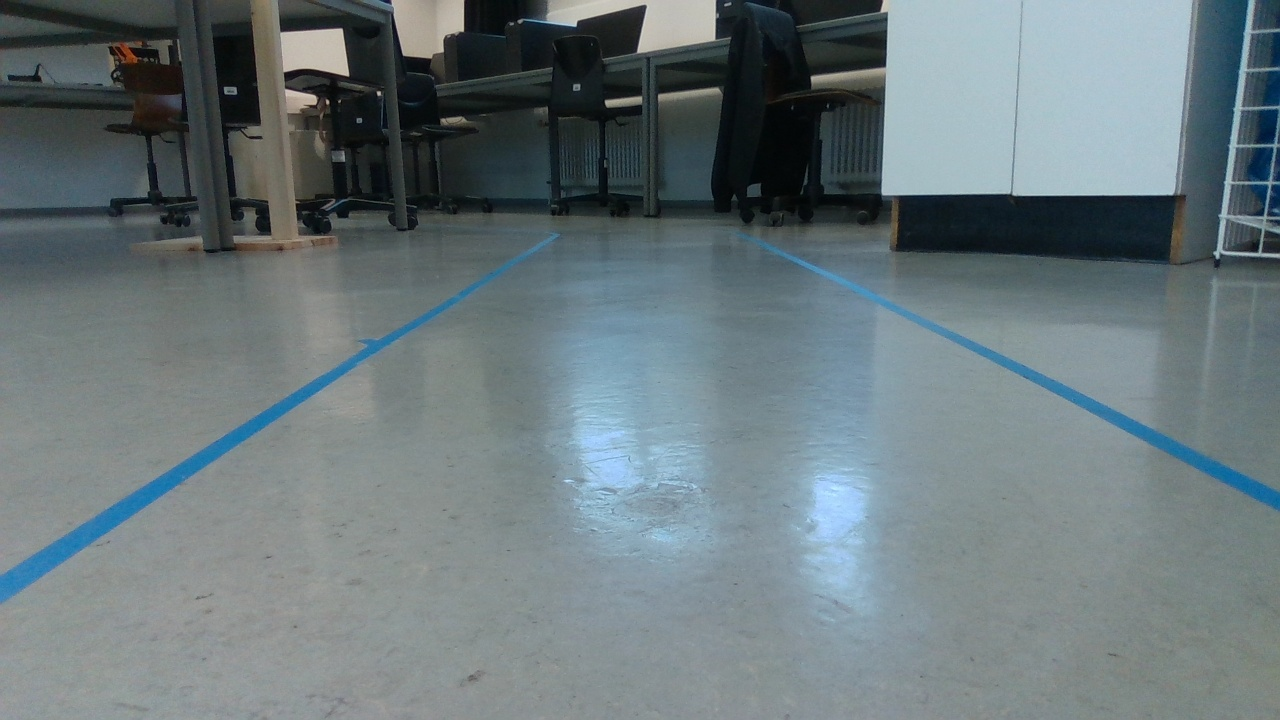
\includegraphics[width=\linewidth]{Laborbedingungen.jpg}
                    \caption{Laborbedingungen}
                    \label{fig:Laborbedingungen}
                \end{figure}

            % ToDo: Beschreiben wie entpackt werden muss

            \subsubsection{Backbone}
                Als Backbone für die verschiedenen Architekturen standen die nachfolgend beschriebenen  Varianten im lanedet-Repository zur Verfügung. Aufgrund von lange anhaltenden Performanceproblemen wurde hauptsächlich das MobileNetV2-Backbone verwendet. In späteren Tests auf dem neuen performanteren Jetson wurde festgestellt, dass auch das ResNet-Backbone in den Größen 18 und 34 verwendet werden kann, ohne die Anforderung von 60ms Interferenzzeit zu überschreiten.

                \textbf{ResNet}, insbesondere ResNet50 und ResNet101, sind bekannt für ihre hohe Genauigkeit bei der Objekterkennung, was sie zu einer beliebten Wahl für Aufgaben im Bereich des autonomen Fahrens macht. ResNet50 bietet eine gute Balance zwischen Präzision und Geschwindigkeit, während ResNet101 eine höhere Genauigkeit auf Kosten eines höheren Speicherverbrauchs und einer größeren Anzahl von Parametern bietet. ResNet-Modelle sind jedoch speicherintensiv und benötigen mehr Rechenleistung, was sie weniger geeignet für mobile oder eingebettete Anwendungen macht.
                \cite{Chen2021Deep}

                \textbf{MobileNetV2}
                MobileNetV2 ist für seine Effizienz und Geschwindigkeit bekannt, was es ideal für Anwendungen auf mobilen und eingebetteten Geräten macht. Es bietet eine schnellere Inferenzgeschwindigkeit im Vergleich zu ResNet, jedoch mit einer etwas geringeren Genauigkeit. MobileNetV2 ist besonders vorteilhaft, wenn die Rechenressourcen begrenzt sind, da es weniger Speicher benötigt und eine leichtere Architektur hat1. In Multi-Task-Learning-Architekturen zeigt MobileNetV2 die schnellste Inferenzgeschwindigkeit, obwohl die Leistung in allen Aufgaben relativ niedriger ist.
                \cite{Chen2021Deep} \cite{Abdigapporov2022Performance}

                \textbf{RESA} (Residual Spatial Attention) ist allgemein bekannt für seine Fähigkeit, die räumliche Aufmerksamkeit in neuronalen Netzen zu verbessern. Es wird oft in Kombination mit anderen Backbones verwendet, um die Leistung bei der Spurerkennung zu verbessern, indem es die relevanten Merkmale in den Eingabedaten besser hervorhebt. RESA kann die Genauigkeit von Modellen erhöhen, indem es die Aufmerksamkeit auf wichtige Bereiche der Eingabebilder lenkt, was besonders nützlich für die Spurerkennung in autonomen Fahranwendungen ist.

                %Todo: Auswahl begründen
                
            \subsubsection{Architekturen}
                Für die verschiedenen Architekturen standen im lanedet-Repository verschiedene Konfigurationen zur Verfügung, die nachfolgend kurz zusammengefasst werden.

                \textbf{Condlane} (\textit{Conditional Lane Detection}) ist eine Architektur, die sich auf die Erkennung von Fahrspuren mit komplexen Topologien, wie z.B. dichte, gekrümmte und verzweigte Linien spezialisiert hat. Diese Architektur nutzt Conditional-Shape-Decoder-Konzept, bei dem die Spur als ein diskretes Set von Punkten repräsentiert wird. Die Spurerkennung wird durch konditionierte Dekodierung basierend auf einem Feature-Extraktionsprozess ermöglicht. Die Stärken von Condlane liegen in der robusten Erkennung von Fahrspuren selbst in komplexen Szenarien wie starken Okklusionen und dichten Linien.
                \cite{Ganeriwala2023Cross}

                \textbf{LaneATT} (\textit{Lane Attention Network}) ist eine Architektur, die sich auf die Effizienz und Genauigkeit der Fahrspurerkennung konzentriert. Sie verwendet einen Aufmerksamkeitsmechanismus, um wichtige Merkmale zu verstärken und die globale Kontextinformation zu erfassen. Der Anwendungsbereich liegt vor allem in strukturierten Umgebungen, bei denen eine hohe Genauigkeit gefordert ist. 
                \cite{He2021Fast}

                \textbf{RESA} (\textit{Recurrent Feature-Shift Aggregator}) ist eine Architektur, die darauf abzielt, Fahrspuren in komplexen Szenarien präzise zu erkennen. Sie nutzt eine rekurrente Verschiebung von Merkmalen, um die räumlichen Beziehungen von Pixeln zu erfassen und globale Informationen zu sammeln. RESA kombiniert grob- und feindetaillierte Merkmale in der Hochskalierungsphase, um eine pixelgenaue Vorhersage zu ermöglichen.
                \cite{Zheng2020RESA}

                \textbf{SCNN} (\textit{Spatial-Temporal Convolutional Neural Network}) ist eine Architektur, die räumlich-zeitliche Informationen nutzt, um die Erkennung von Fahrspuren zu verbessern. Sie verwendet ein Encoder-Decoder-Framework und integriert räumlich-zeitliche rekurrente Module, um zusammenhängende Informationen aus Bildsequenzen zu extrahieren. SCNN zeigt eine hohe Genauigkeit und Effizienz in Echtzeitszenarien.
                \cite{Li2024Enhanced}

                \textbf{UFLD} (\textit{Ultra Fast Lane Detection}) ist eine Architektur, die auf Geschwindigkeit und Effizienz optimiert ist. Sie verwendet eine Bottom-Up-Strategie, um Fahrspuren schnell zu erkennen, und zeigt eine hohe Leistung auf gängigen Datensätzen wie CULane und TuSimple. UFLD ist bekannt für seine Fähigkeit, schnell und mit hoher Genauigkeit zu arbeiten.
                \cite{Xu2024Exploring}

            \subsubsection{Konfigurationsauswahl}
                Nach subjektiver Bewertung der verschiedenen Modelle wurde sich für das Modell mit dem Mobile-Net Backbone und der Architektur laneatt in Kombination mit dem TUSimple Datensatz entschieden, da dort zunächst die besten Spurerkennungen erzielt werden konnten.
                In späteren Tests konnten die zunächst subjektiv ausgewählten Kriterien auch mit Zahlen belegt werden, wie Abbildung \ref{fig:Modell_Auswertung} zeigt.
                Die spalte BestMetric ist dabei mit dem F1-Score gleichzusetzen, der während der Validierung der Modelle berechnet wird.
                %Todo: F1-Score erklären?
                \begin{figure}[h!]
                    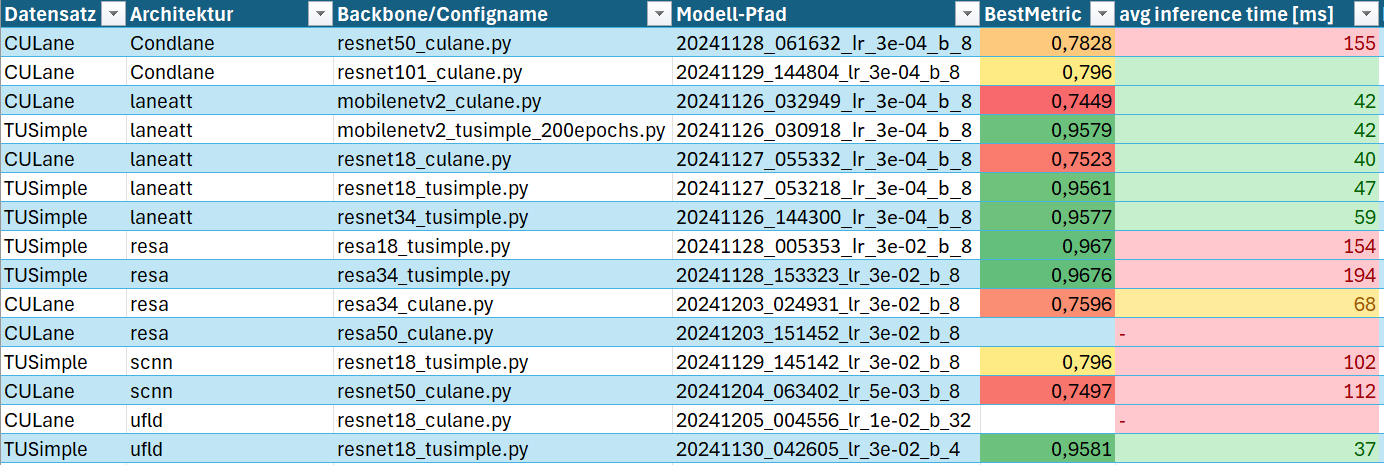
\includegraphics[width=\linewidth]{Auswertung_BackBone_Datensatz.png}
                    \caption{Modell-Auswertung}
                    \label{fig:Modell_Auswertung}
                \end{figure}
                Wie die Grafik aufzeigt, ist der TUSimple-Datensatz mit einem F1-Score von etwa 0.95 dem CULane-Datensatz mit einem Wert von etwa 0.75 deutlich überlegen, was durch die schwierigeren Bedingungen des CULane-Datensatzes zu erklären ist. Da in den Laborbedingungen des HTWG-RaceCars jedoch keine solch schwierigen Bedingungen wie Okklusionen vorliegen, ist der TU-Simple Datensatz für die Spurerkennung besser geeignet.

        \subsection{Performance}
            % --> performance der modelle auf Labor PC's
            % --> performance der Modelle auf altem Jetson

            % Todo Performance in Bildern/Excel zeigen
            
            Erste Tests auf dem Jetson Nano zeigten jedoch, dass die Modelle nicht in Echtzeit betrieben werden konnten. Eine anfängliche Verarbeitszeit von etwa 20 Sekunden pro Bild war deutlich zu langsam.
            In der Analyse wurde festgestellt, dass die größte Bottleneck im versenden der Bilder zwischen ROS-Knoten in der ROS-Version lag. In der Version Foxy gab es für python bekannte Performance Probleme wie dieser Issue zeigt: \url{https://github.com/ros2/rclpy/issues/763}.
            In neuen Tests mit ROS2 Humble und einer präziseren Messung der Interferenz-Zeit lag die Verarbeitungszeit bei etwa einer Sekunde pro Bild, was immernoch zu langsam war.
            Um dieses Problem zu lösen wurde versucht das Modell zu quantisieren, was jedoch nicht zum Erfolg führte.
            Eine Konvertierung in das ONNX-Format, konnte zwar durchgeführt werden, allerdings erkannte das konvertierte Modell keine Spurmarkierungen mehr.
            %Todo mehr ausführen @Mars?
            Nach anschaffung eines neuen Jetson Nano konnte die Performance des Modells auf dem Jetson Nano deutlich verbessert werden, sodass keine weitere Anpassung mehr nötig waren.
            Auf diesem Jetson läuft nach letztem Stand ROS2 in der Version IRON und erzielt die in \ref{fig:Modell_Auswertung} gezeigten Interferenz-Zeiten mit Bestwerten um 40ms.

            Die Erkennung der Spurmarkierungen funktionierte nun bereits sehr robust wie folgende Abbildung zeigt.
            Die gelabelten Spurmarkierungen sind in orange/grünen Kreuzen dargestellt, während die vom Modell erkannten Spurmarkierungen in lila/blauen Punkten dargestellt sind.
            \begin{figure}[h!]
                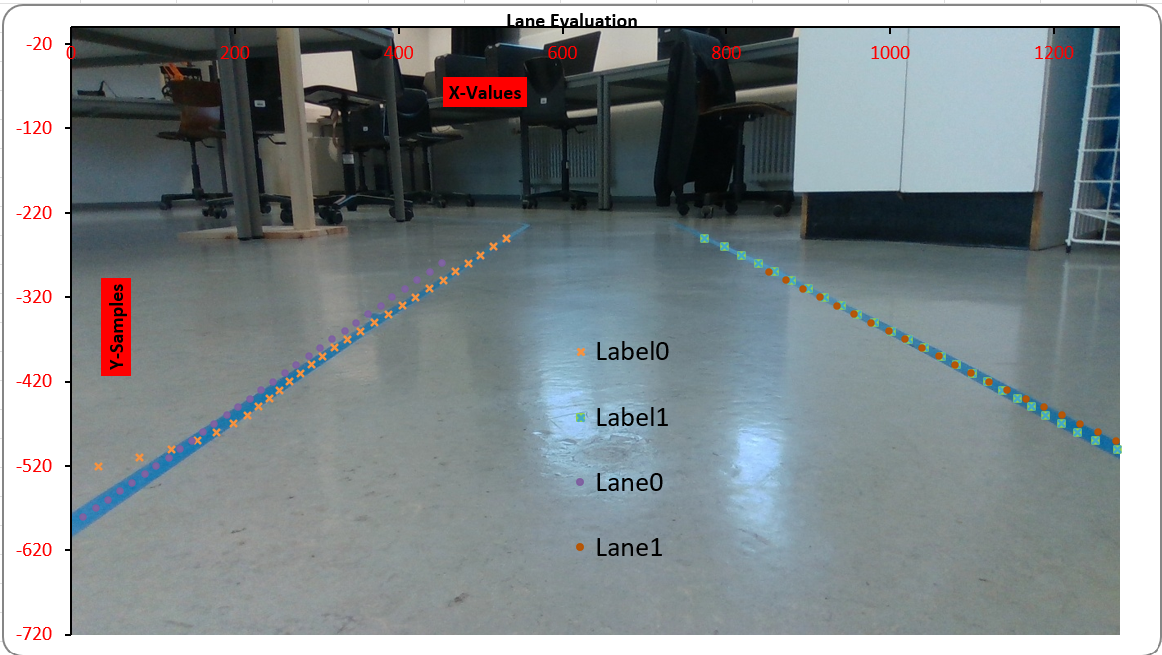
\includegraphics[width=\linewidth]{Auswertung_6e7e3724-test_103.png}
                \caption{Auswertung 6e7e3724-test103.png}
                \label{fig:Auswertung_6e7e3724-test_103.png}
            \end{figure}
            Die folgende Abbildung \ref{fig:AbsoluterFehlerCm} zeigt den Verlauf des Absoluten Fehlers in cm abhängig von der y-Koordinate des Bildes auf.
            Dieser wurde berechnet, indem die bekannte Distanz zwischen den Spurmarkierungen von 60cm mit der Distanz zu den erkannten Spurmarkierungen verglichen wurde.

            \begin{equation}
                 c = \frac{D}{d} \cdot l
            \end{equation}
            Dabei ist $c$ der absolute Fehler in cm, $D$ die bekannte Distanz zwischen den Spurmarkierungen (60cm), $d$ die Distanz zwischen den gelabelten Spurmarkierungen in Pixeln und $l$ die Distanz zwischen gelabelter Linie und erkannter Linie in Pixeln.

            \begin{figure}[h!]
                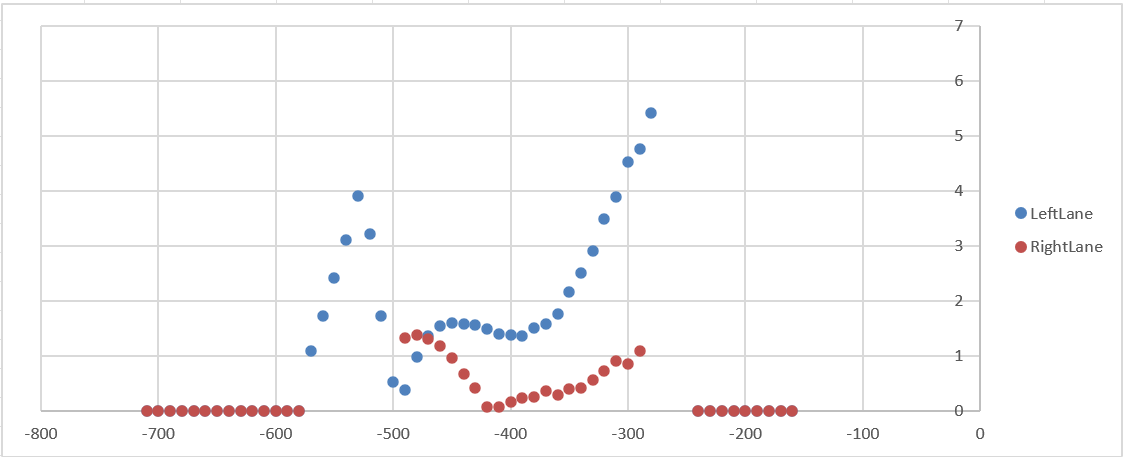
\includegraphics[width=\linewidth]{Auswertung_6e7e3724-test_103_absolut.png}
                \caption{Absoluter Fehler in cm}
                \label{fig:AbsoluterFehlerCm}
            \end{figure}

            Wie auf in Abbildung \ref{fig:AbsoluterFehlerCm} zu erkennen ist liegt der absolute Fehler in cm bei maximal 6cm und im Durchschnitt bei knapp unter 2cm, was eine sehr gute Genauigkeit darstellt.
            Der erste Peak bei etwa -500 ist durch eine ungenauigkeit im Label0 zu erklären, die während der Umrechnung von den tatsächlich gelabelten Punkten auf die von TUSimple hart kodierten y-Samples entstanden ist. 
            Abgesehen davon ist im Trend erkennbar, dass der absolute Fehler in cm mit zunehmender y-Koordinate zunimmt, was durch die Perspektive des Bildes zu erklären ist.
            Die 0-Werte am Ende des Bildes sind durch zu kurze erkannte Linien zu erklären, die nicht bis zum Ende des Bildes reichen.


        %\subsection{Steuerung}
            % alte Steuerung
            % Projekt während Autonomes Fahren --> neue Knotenaufteilung
            % neue Steuerung
    \section{Fazit}
        \subsection{Ergebnisse}
        Im folgenden Abschnitt werden die Ergebnisse des Projekts zusammengefasst und bewertet. Die Abbildungen %Todo: Referenzen
        zeigen die von der KI erkannten Spurmarkierungen in lila/blau und die von der Kantendetektion erkannten Spurmarkierungen in orange/grün.
        Wie Abbildung Todo zeigt, ist die Erkennung der Spurmarkierungen unter idealen Bedingungen in beiden Systemen sehr gut.
        Der Unterschied zwischen den beiden Systemen zeigt sich jedoch in der Robustheit gegenüber schwierigen Bedingungen. So hatte die Kantendetektion Probleme mit Schatten und Spiegelungen, während die KI diese Probleme deutlich besser bewältigen konnte, wie Abbdilung Todo zeigt.
        Damit wurde das Projektziel erreicht, eine zuverlässige Spurerkennung auch unter schwierigen Bedingungen zu ermöglichen. Auch die Echtzeitfähigkeit des Systems konnte durch den Einsatz eines neuen Jetson Nano erreicht werden, bei dem die Interferenz-Zeiten unter 60ms liegen.
        \subsection{Probleme}
        Entgegen der ersten Annahme, dass der Einsatz KI-basierter Spurerkennung die Gesamt-Performance des autonomen Steuerungssystems verbessern würde, konnte dies nicht bestätigt werden.
        Als Hauptproblem wurde der Schritt zwischen erkannten Linien und Steuerung identifiziert. Auch wenn die Spurmarkierungen sehr genau erkannt wurden, war die Steuerung des Fahrzeugs nicht immer zuverlässig, sodass die Spur verlassen wurde. Sobald dann nur noch eine Spurmarkierung erkannt wurde, konnte das Fahrzeug nur selten in die Spur zurückgeführt werden.
        Als Hauptproblem wurde die sehr starke Vereinfachung von zwei Spurmarkierungen auf eine senkrechte CenterLine identifiziert.
        Diese bildet die reale Situation zu ungenau ab, sodass das Fahrzeug nicht immer in der Spur gehalten werden konnte.

        \subsection{Ausblick}
        Für eine bessere Steuerung des Fahrzeugs sollte die Spurerkennung um eine Spurfolge erweitert werden, um im Falle des Verlassens der Spur das Fahrzeug wieder in die Spur zu führen. So könnte besser interpretiert in welche Richtung das Fahrzeug die Spur verlassen hat und entsprechend gegengesteuert werden.
        Außerdem sollte die Steuerung die volle Information aus den erkannten Spurmarkierungen nutzen, um das Fahrzeug besser in der Spur zu halten. So könnte zum Beispiel eine Mittellinie zwischen den beiden erkannten Spurmarkierungen berechnet werden, bei der es sich nicht mehr um eine senkrechte Linie handelt, sondern mindestens aktuellen Winkel der Spurmarkierungen berücksichtigt. Idealerweise könnte ein Polynom höheren Grades verwendet werden, um auch Kurven besser abzubilden und die Steuerung vorausschauender zu gestalten.


\end{document}